% Options for packages loaded elsewhere
\PassOptionsToPackage{unicode}{hyperref}
\PassOptionsToPackage{hyphens}{url}
%
\documentclass[
]{article}
\title{Measuring Polarization in Online Communities\thanks{The code for this project is hosted on GitHub at \href{https://github.com/wlgfour/social_networks}{wlgfour/social\_networks}}}
\usepackage{etoolbox}
\makeatletter
\providecommand{\subtitle}[1]{% add subtitle to \maketitle
  \apptocmd{\@title}{\par {\large #1 \par}}{}{}
}
\makeatother
\subtitle{using exponential family random graph models and sentiment analysis}
\author{William Gerecke}
\date{29 April 2022}

\usepackage{amsmath,amssymb}
\usepackage{lmodern}
\usepackage{iftex}
\ifPDFTeX
  \usepackage[T1]{fontenc}
  \usepackage[utf8]{inputenc}
  \usepackage{textcomp} % provide euro and other symbols
\else % if luatex or xetex
  \usepackage{unicode-math}
  \defaultfontfeatures{Scale=MatchLowercase}
  \defaultfontfeatures[\rmfamily]{Ligatures=TeX,Scale=1}
\fi
% Use upquote if available, for straight quotes in verbatim environments
\IfFileExists{upquote.sty}{\usepackage{upquote}}{}
\IfFileExists{microtype.sty}{% use microtype if available
  \usepackage[]{microtype}
  \UseMicrotypeSet[protrusion]{basicmath} % disable protrusion for tt fonts
}{}
\makeatletter
\@ifundefined{KOMAClassName}{% if non-KOMA class
  \IfFileExists{parskip.sty}{%
    \usepackage{parskip}
  }{% else
    \setlength{\parindent}{0pt}
    \setlength{\parskip}{6pt plus 2pt minus 1pt}}
}{% if KOMA class
  \KOMAoptions{parskip=half}}
\makeatother
\usepackage{xcolor}
\IfFileExists{xurl.sty}{\usepackage{xurl}}{} % add URL line breaks if available
\IfFileExists{bookmark.sty}{\usepackage{bookmark}}{\usepackage{hyperref}}
\hypersetup{
  pdftitle={Measuring Polarization in Online Communities},
  pdfauthor={William Gerecke},
  pdfkeywords={Social networks, Exponential family Random Graph Model, ERGM, Polarization, Sentiment analysis},
  hidelinks,
  pdfcreator={LaTeX via pandoc}}
\urlstyle{same} % disable monospaced font for URLs
\usepackage[margin=1in]{geometry}
\usepackage{longtable,booktabs,array}
\usepackage{calc} % for calculating minipage widths
% Correct order of tables after \paragraph or \subparagraph
\usepackage{etoolbox}
\makeatletter
\patchcmd\longtable{\par}{\if@noskipsec\mbox{}\fi\par}{}{}
\makeatother
% Allow footnotes in longtable head/foot
\IfFileExists{footnotehyper.sty}{\usepackage{footnotehyper}}{\usepackage{footnote}}
\makesavenoteenv{longtable}
\usepackage{graphicx}
\makeatletter
\def\maxwidth{\ifdim\Gin@nat@width>\linewidth\linewidth\else\Gin@nat@width\fi}
\def\maxheight{\ifdim\Gin@nat@height>\textheight\textheight\else\Gin@nat@height\fi}
\makeatother
% Scale images if necessary, so that they will not overflow the page
% margins by default, and it is still possible to overwrite the defaults
% using explicit options in \includegraphics[width, height, ...]{}
\setkeys{Gin}{width=\maxwidth,height=\maxheight,keepaspectratio}
% Set default figure placement to htbp
\makeatletter
\def\fps@figure{htbp}
\makeatother
\setlength{\emergencystretch}{3em} % prevent overfull lines
\providecommand{\tightlist}{%
  \setlength{\itemsep}{0pt}\setlength{\parskip}{0pt}}
\setcounter{secnumdepth}{5}
\newlength{\cslhangindent}
\setlength{\cslhangindent}{1.5em}
\newlength{\csllabelwidth}
\setlength{\csllabelwidth}{3em}
\newlength{\cslentryspacingunit} % times entry-spacing
\setlength{\cslentryspacingunit}{\parskip}
\newenvironment{CSLReferences}[2] % #1 hanging-ident, #2 entry spacing
 {% don't indent paragraphs
  \setlength{\parindent}{0pt}
  % turn on hanging indent if param 1 is 1
  \ifodd #1
  \let\oldpar\par
  \def\par{\hangindent=\cslhangindent\oldpar}
  \fi
  % set entry spacing
  \setlength{\parskip}{#2\cslentryspacingunit}
 }%
 {}
\usepackage{calc}
\newcommand{\CSLBlock}[1]{#1\hfill\break}
\newcommand{\CSLLeftMargin}[1]{\parbox[t]{\csllabelwidth}{#1}}
\newcommand{\CSLRightInline}[1]{\parbox[t]{\linewidth - \csllabelwidth}{#1}\break}
\newcommand{\CSLIndent}[1]{\hspace{\cslhangindent}#1}
\usepackage{booktabs}
\usepackage{longtable}
\usepackage{array}
\usepackage{multirow}
\usepackage{wrapfig}
\usepackage{float}
\usepackage{colortbl}
\usepackage{pdflscape}
\usepackage{tabu}
\usepackage{threeparttable}
\usepackage{threeparttablex}
\usepackage[normalem]{ulem}
\usepackage{makecell}
\usepackage{xcolor}
\ifLuaTeX
  \usepackage{selnolig}  % disable illegal ligatures
\fi

\begin{document}
\maketitle
\begin{abstract}
With the growth of the internet and social media platforms, it is increasingly easy for communities of like-minded people to form. This can be good, but often results in people strengthening beliefs by affirmation rather than by a decision making process. In this paper, I use Exponential Random Graph Models and sentiment analysis to measure polarization in online communities, specifically on the site Reddit. I find some evidence that indicates a diversity of opinions being expressed in several communities. However, it is still important for companies that make social media sites as well as individuals using the sites to consider the impact of forming homogeneous communities in the future.

\par

\textbf {Keywords:} Social networks, Exponential family Random Graph Model, ERGM, Polarization, Sentiment analysis
\end{abstract}

\newpage
\tableofcontents

\newpage

\hypertarget{introduction}{%
\section{Introduction}\label{introduction}}

With the popularization of the internet, and increasing ease of access, social media is becoming ubiquitous in modern society. These platforms facilitate instant communication between individuals, or between an individual and large audience. Beyond the ease and availability of such communication, social media platforms are run by highly-engineered algorithms that are designed to find people and communities that are similar to each other. For people like hobbyists, this is good since it allows people from niche groups to find each other easily. It is possible, however, to see that this could have a polarizing effect in a different scenario. For example, people with political beliefs are presented with like-minded opinions from around the world, and such communities strengthen their beliefs by affirmation, rather than by a decision making process. As such, it is important to be able to measure and understand the effect that online communities have on the people that participate in them, and the behaviors exhibited therein

Many social media platforms can be represented as graphs, as they represent an underlying social network of individuals. Graphs are data structures that are represented by a set of nodes \(V\) and a set of edges \(E\subseteq\{(x,y)\in V^2,x\not=y\}\) which represent a connection between nodes. There are countless phenomena that can be represented by this data structure, such as roads, mathematical operations, supply chains, the internet, social networks, and more. As such, understanding and modelling graphical structures is crucial to understanding the universe that we live in, and has been a topic of much research. The problem with graphical structures is that typical assumptions of independence are violated by many of the scenarios that are represented by graphs. For example, in a social network where people share an edge if they are friends, the probability of sharing an edge is no longer independent. This is because it is reasonable that sharing a mutual friend will influence the probability of a friendship. Statisticians have developed Exponential family Random Graph Models (ERGMs) in order to allow for the representation of these dependent relationships.

In this paper, I look at polarization in online communities, specifically on the social media platform Reddit. For the purpose of this paper, I define polarization as the tendency for people to respond positively in the presence of positive sentiments, and negatively in the presence of negative sentiments. That is, polarization is defined to be when individuals in a community have views and opinions that align. I use a graph to represent interactions within communities on the Reddit, and sentiment analysis to classify individual interactions as positive or negative. I find some evidence that indicates that differing opinions are being expressed on several popular Reddit communities, but highlight the fact that a better construction of the underlying data would yield more conclusive results.

I begin by describing how the data is gathered, cleaned, and parsed into a graphical structure. I proceed to elaborate on the model used for sentiment analysis, and the structure of ERGMs. After that, I discuss the results of applying these models to the data that was gathered in order to measure polarization in online communities. Finally I discuss the impact of the results, weaknesses with the approach presented, and suggest directions for future research.

\hypertarget{data}{%
\section{Data}\label{data}}

\hypertarget{software}{%
\subsection{Software}\label{software}}

The R programming language (R Core Team 2021) was used to generate the report, data, and analyses associated with this project. The \texttt{purrr}, \texttt{dplyr}, \texttt{stringr}, and \texttt{tidyr} were used for data manipulation Wickham (2021). Data was simulated using the \texttt{stringi} and \texttt{keyToEnglish} packages Candocia (2021). The \texttt{VADER}, which exposed an R API for the VADER NLP model was used to generate sentiment labels for the data (Hutto and Gilbert 2014). \texttt{jsonlite} was used to scrape data from Reddit using Reddit's json API (Ooms 2014). The \texttt{statnet} package was used to generate network data structures, as well as fit ERGM models Hunter et al. (2008). Finally, the code and data are hosted on GitHub ({``Where the World Builds Software,''} n.d.).

\hypertarget{reddit}{%
\subsection{Reddit}\label{reddit}}

The site Reddit was used to gather data for this project. Reddit is structured such that there are communities that users can subscribe to called subreddits. When someone creates a post, the post is categorized under a subreddit. Once a post is created, users can then comment on a post, as well as other comments. ``Has-a'' relationships are as follows:

\begin{itemize}
\tightlist
\item
  subreddit: N/A
\item
  post: subreddit, author
\item
  comment: parent (post or comment), subreddit, author
\end{itemize}

That is, a post has a subreddit and author that it is associated with. This project uses a dataset composed of instances of comments which have a parent, author, and subreddit associated with them, in addition to a comment body (text), and other metadata.

\hypertarget{gathering}{%
\subsection{Gathering}\label{gathering}}

Data was gathered using the Reddit json API. Given any Reddit url \texttt{u}, a json string representing that url can be obtained by downloading the url given by \texttt{\{url\}/.json}. The algorithm for scraping comments is as follows:

\begin{enumerate}
\def\labelenumi{\arabic{enumi}.}
\tightlist
\item
  Initialize \texttt{links} to have top posts from some seed communities. Initialize \texttt{comments} to be empty
\item
  Randomly select a \texttt{link} from \texttt{links}
\item
  Append all comments from \texttt{link} to \texttt{comments}
\item
  If \texttt{link} represents a use: add the posts from the users most recent comments to \texttt{links}
\item
  If \texttt{link} represents a post: add the users from the posts comments to \texttt{links}
\item
  Remove duplicates in \texttt{comments} and \texttt{links}. Remove \texttt{links} that have already been visited. Remove rows in \texttt{comments} that contain \texttt{NA} values.
\item
  Goto 2.
\end{enumerate}

At the start of the algorithm, a cache file is generated, and the algorithm caches \texttt{comments} every 10 iterations. For this project, the seed was set to three of the most active subreddits, `AskReddit,' `worldnews,' and `gifs' (reddit 2011).

\begin{table}

\caption{\label{tab:rawdata}The table shows the summary statistics for the 15 subredits with the most comments recorded, and the total summary statistics for all subreddits visited.}
\centering
\begin{tabular}[t]{lrrr}
\toprule
Subreddit & Posts & Unique users & Average replies per comment\\
\midrule
AskReddit & 22,605 & 3,829 & 1.66\\
worldnews & 13,992 & 2,795 & 1.45\\
gifs & 1,521 & 1,125 & 2.76\\
ukraine & 1,492 & 327 & 1.15\\
news & 1,163 & 555 & 1.17\\
\addlinespace
politics & 1,051 & 366 & 1.20\\
AmItheAsshole & 875 & 207 & 1.18\\
funny & 790 & 473 & 1.27\\
interestingasfuck & 788 & 449 & 1.15\\
technology & 763 & 369 & 1.19\\
\addlinespace
movies & 694 & 360 & 1.16\\
Damnthatsinteresting & 644 & 311 & 1.16\\
AskMen & 632 & 204 & 1.25\\
antiwork & 628 & 310 & 1.26\\
mildlyinteresting & 539 & 338 & 1.17\\
\midrule
\addlinespace
Total & 117,437 & 44,108 & 1.02\\
\bottomrule
\end{tabular}
\end{table}

Statistics for the raw data that was gathered can be seen in table \ref{tab:rawdata}. There were 7208 subreddits visited, but the data collected for most of them was fairly sparse. It is important to note that when Reddit returns information, it hides many of the comments in a post by default. It is possible to retrieve the hidden comments by expanding certain links, but I did not do that for this project, which explains why the comment multiplicity is so low, averaging between 1 and 2 in the dataset. We can also see that significantly more comments have been gathered from AskReddit than any other subreddit. This is probably because this was one of the seed communities, and the posts on AskReddit have a high multiplicity. As such, many links were gathered from AskReddit early, making it more likely to gather more links from AskReddit, which in turn makes it more likely to gather even more links from AskReddit. This is an artifact of the algorithm that I used to scrape data, and the report would benefit from designing an algorithm that does not have this weakness.

\hypertarget{cleaning}{%
\subsection{Cleaning}\label{cleaning}}

Once the data scraping script is run, and there are one or more chunks of raw data, the data are combined, filtered, and labelled with sentiment scores. Due to computational constraints, the amount of data that was processed had to be severely limited. The first computational constraint came from generating sentiment scores, which is a very computationally intensive process. The second is fitting the model, and assessing its goodness of fit, which was another source of significant computational burden. Even with ample time, R experienced frequent crashes, indicating that in order to perform analyses on the entire dataset or a larger sample, better software design is important.

The filtering process excluded portions of the data for two reasons. One is because there weren't enough data points, and the second is because there were too many data points for the analyses to be computationally feasible. Data were first gathered and grouped by subreddit. Then data from a subreddit with fewer than 500 recorded comments were dropped. Finally, if a subreddit had more than 1000 recorded comments, 1000 were selected at random.

The sentiment scoring process was the main computational bottleneck in the data preparation process. With better software design, the process cold be parallelized to greatly speed up the labeling process and allow for larger datasets. This, however, would likely need to be done outside of the R language because even when run using only one thread on about 20,000 comments, the R garbage collection process caused the program to crash repeatedly.

\begin{table}

\caption{\label{tab:cleanstats}The table shows the summary statistics for the 15 subredits with the most comments recorded, and the total summary statistics for all subreddits visited.}
\centering
\begin{tabular}[t]{lrrrr}
\toprule
Subreddit & Posts & Unique users & Average replies per comment & Avg. sentiment\\
\midrule
AskReddit & 1,000 & 771 & 1.20 & 0.03\\
gifs & 1,000 & 783 & 2.54 & 0.20\\
news & 1,000 & 512 & 1.16 & -0.02\\
AmItheAsshole & 875 & 207 & 1.18 & 0.09\\
funny & 790 & 473 & 1.27 & 0.07\\
\addlinespace
interestingasfuck & 788 & 449 & 1.15 & 0.06\\
movies & 694 & 360 & 1.16 & 0.12\\
Damnthatsinteresting & 644 & 311 & 1.16 & 0.07\\
AskMen & 631 & 204 & 1.25 & 0.13\\
antiwork & 628 & 310 & 1.26 & 0.04\\
\addlinespace
mildlyinteresting & 539 & 338 & 1.17 & 0.06\\
Eldenring & 537 & 120 & 1.10 & 0.00\\
gaming & 515 & 298 & 1.11 & 0.12\\
memes & 503 & 229 & 1.10 & 0.05\\
politics & 54 & 44 & 1.04 & 0.03\\
\midrule
\addlinespace
Total & 10,198 & 5,409 & 1.26 & 0.07\\
\bottomrule
\end{tabular}
\end{table}

\begin{figure}

{\centering 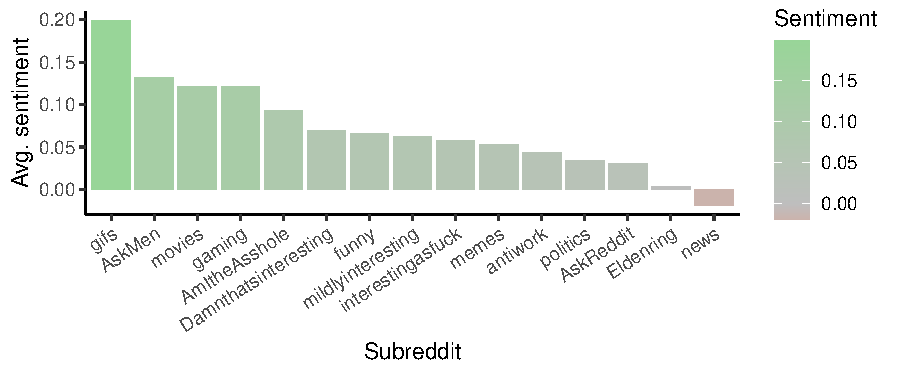
\includegraphics{E:/School/STA304/social_networks/outputs/report/report_files/figure-latex/sentchart-1} 

}

\caption{Average sentiment expressed in comments on each subreddit that was included in the cleaned dataset.}\label{fig:sentchart}
\end{figure}

In table \ref{tab:cleanstats}, we can see the information for the 15 subreddits that were included in the cleaned dataset. As we can see, the subreddits have between 500 and 1000 comments each, with some subreddits having significantly more unique users. This is most likely due to the random sample that was taken for groups that had more than 1,000 comments. We can also see that the subreddits that were sampled are significantly sparser than they were before the sampling. A better sampling operation that preserves the structure of the comment chains could be advantageous when fitting models to represent the interactions that are present. We can see that there is one subreddit with only 54 values in the cleaned data. This is because the script that cleaned the data and labeled the sentiments always crashed before labeling all of the sentiments.

Figure \ref{fig:sentchart} shows the average sentiments of the comments that were gathered for each subreddit. We can see that overall, most of the comments are slightly positive, but mostly neutral, with very few negative comments relative to positive comments. Beyond that, we can see that news and EldenRing have the lowest average sentiment scores, with gifs having a much higher average score.

\hypertarget{graph-construction}{%
\subsection{Graph construction}\label{graph-construction}}

In order to create the graphical representation of the data, it was important to develop a scheme that represented the underlying structure of interactions that are present in the online conversations gathered. Several different approaches were considered, and the one that was selected is outlined below. It is important to note that there is likely a better design that allows for better representations of the data. It is also important to note that the way the graph is constructed directly influences how accurately it represents the network as well as the computational feasibility of the models that operate over the graphical representations.

\begin{figure}

{\centering 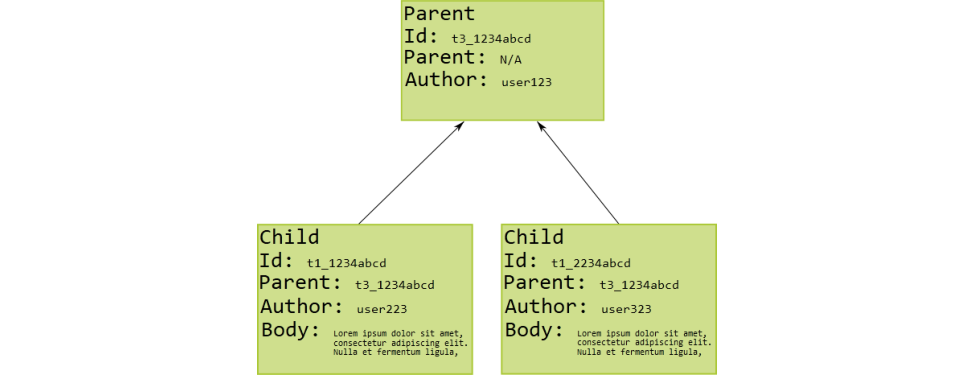
\includegraphics{E:/School/STA304/social_networks/outputs/report/report_files/figure-latex/graph-1} 

}

\caption{The figure shows the relationships expressed by the graphical construction used by this project. Each square represents a node, and the text contained within represents the attributes associated with each node. The parent in this case represents a post, and would not have a body, but it could also be a comment.}\label{fig:graph}
\end{figure}

Figure \ref{fig:graph} describes the graphical structure that is used in this project. Consider the data examined by this project to be a social network. Social networks can be represented as a graph with nodes \(V\) and edges \(E\subseteq V\times V\). I decided to use a directed graph where each node represents a post or comment. Nodes have an associated sentiment, author, subreddit, parent, and ID as seen below:

\begin{verbatim}
    node <- {
      .sentiment
      .author
      .subreddit
      .parent
      .id
    }
\end{verbatim}

There are two constraints on the nodes:

\begin{enumerate}
\def\labelenumi{\arabic{enumi}.}
\tightlist
\item
  \(node.sentiment\in[-1,1]\)
\item
  \(\{node.parent|node\in V\}\equiv \{node.id|node\in V\}\)
\end{enumerate}

\begin{table}

\caption{\label{tab:graphstats}The table shows the descriptive statistics of the graphs that represent the data collected for each subreddit.}
\centering
\begin{tabular}[t]{lrrr}
\toprule
Subreddit & Nodes & Edges & Density\\
\midrule
AmItheAsshole & 1,617 & 875 & 3e-04\\
antiwork & 1,617 & 875 & 3e-04\\
AskMen & 1,617 & 875 & 3e-04\\
AskReddit & 1,617 & 875 & 3e-04\\
Damnthatsinteresting & 1,617 & 875 & 3e-04\\
\addlinespace
Eldenring & 1,617 & 875 & 3e-04\\
funny & 1,617 & 875 & 3e-04\\
gaming & 1,617 & 875 & 3e-04\\
gifs & 1,617 & 875 & 3e-04\\
interestingasfuck & 1,617 & 875 & 3e-04\\
\addlinespace
memes & 1,617 & 875 & 3e-04\\
mildlyinteresting & 1,617 & 875 & 3e-04\\
\bottomrule
\end{tabular}
\end{table}

Exceptions to these rules are posts themselves, since top level comments are all direct children of posts, which do not have a parent or sentiment. In this case, \(parent.parent=NA\), and is not included in the graph. The result of this is that comment chains will appear as inverted trees.

Since the graph is directional, the existence of an edge \((u,v)\in E\) does not guarantee the existence of edge \((v,u)\). In fact, because comments on Reddit form a tree, and each comment can only be a reply to one parent, this explicitly guarantees that \((v,u)\not\in E\). Another side effect of the fact that each node will only originate one edge is that the graph will be very sparse, with \(|E|\in\mathcal{O}(V)\).

Furthermore, I define one graph for each subreddit, \(sub\), as the graph over the nodes \(V_{sub}\equiv\{n|n.subreddit=sub,\ n\in V\}\). Note that there are no edges that need to be severed due to this construction because any comment will explicitly be a reply to some media that was posted in that subreddit. Thus, \(G_{sub}=(V_{sub},E_{sub})\) is a straightforward construction.

Table \ref{tab:graphstats} shows the statistics for the graphs constructed for each subreddit. We can see that the graphs are extremely sparse. This is because of the fact that I did not expand the comments that were hidden when scraping data. This is also due to the fact that I had to sample the data during the cleaning process, and I did it in a way that did not preserve comment chains which resulted in the artifact shown in the table. This is supported by the fact that the subreddits that were subsampled to a lower proportion of the total data collected have a lower density.

\hypertarget{model}{%
\section{Model}\label{model}}

\hypertarget{sentiment-analysis}{%
\subsection{Sentiment Analysis}\label{sentiment-analysis}}

Sentiment analysis was done using the VADER (Valance Aware Dictionary for sEntiment Reasoning) model from NLP that was specifically designed to perform well on content from the internet (Hutto and Gilbert 2014). VADER is capable of identifying polarity and intensity of the sentiment expressed by text and returns a composite sentiment score between -1 and 1, where -1 represents a strong negative sentiment, 0 is neutral, and 1 represents a strong positive sentiment.

VADER uses a dictionary to identify lexical fragments and assign sentiment scores (intensity and polarity) to components of the body of text. The dictionary that maps lexical features to sentiment scores was trained using manually labeled data. VADER is also capable of understanding contextualization such as ``I don't like this,'' as well as non-standard contractions such as ``like'nt'' by using some simple heuristics that the authors decided on. The scores assigned to lexical components are then averaged, and normalized.

\hypertarget{ergm}{%
\subsection{ERGM}\label{ergm}}

The model used to understand the graphical structure of the data which is examined in this report is the ERGM. This is because typical statistical models assume that the observations that they operate over are independent of each other. For example, if two people are friends on a social network, they are more likely to interact with each others' media, hence increasing the probability of an edge between them, and invalidating the assumption that they are independent of each other. In order to account for the dependence between the observations, we need to use a model that takes into account the underlying representation of the dataset. The ERGM is analogous to the generalized linear model, but takes into account the underlying structure of the graph, which is why it's appropriate for this application.

Given an observed network, the ERGM estimates the parameters of an expontential family model that takes the form of a log-linear combination of feature weights (Wyatt, Choudhury, and Bilmes 2009): \[
p(\mathbf{Y}=y)=\frac{1}{Z_\eta}{e^\eta}^\top\phi(y)
\]

Where:

\begin{itemize}
\tightlist
\item
  \(\mathbf{Y}\) are weights representing the edges of the graph
\item
  \(\phi\) defines the features over \(y\)
\item
  \(\eta\) is a vector of weights
\item
  \(Z_\eta\) is a normalizing constant
\end{itemize}

Typically, features account for the structural dependencies int he graph, allowing the model to more intuitively reason over the graphical structure of the data. The problem with using these models in practice, though, is that models are highly prone to degeneracy. In order to assess model degeneracy, it is important to examine the goodness of fit (GOF) which uses the generative nature of the estimated ERGM to find simulated networks. The simulated networks are then used to provide estimates for features such as node degree, edgewise shared partners, and geodesic distance. If the estimated networks align with the observed network, the model can be said to be robust.

\hypertarget{results}{%
\section{Results}\label{results}}

In order to assess polarity in the dataset that I gathered, I fit an ERGM model to the graph that represents each subreddit. For model features, I used the sentiment covariances, as well as basic geometric predictors that are present in the graph, such as edges which is equivalent to using the mean in a linear model. The idea between using the covariance associated with the sentiment score is that if the sentiment score covariance is found to have a positive impact on the formation of an edge, then this indicates that comments are likely to be replies to like-minded comments. That is, comments are more likely to be replies to comments that express the same sentiment. Similarly, a negative impact on edge formation signifies that comments are more likely to disagree with each other. In other words, if a comment expresses a positive sentiment, it is likely to receive a negative reply.

\begin{table}

\caption{\label{tab:modelstats}The table shows the estimated parameters for the models fit to each subreddit graph as well as their confidence levels.}
\centering
\begin{tabular}[t]{lrrrr}
\toprule
Subreddit & Edges & Pr(edges>|z|) & Sentiment cov. & Pr(cov(sentiment)>|z|)\\
\midrule
AmItheAsshole & -8.00 & 0 & -0.02 & 0.706\\
antiwork & -7.61 & 0 & -0.02 & 0.821\\
AskMen & -7.61 & 0 & -0.06 & 0.445\\
AskReddit & -8.11 & 0 & -0.02 & 0.791\\
Damnthatsinteresting & -7.70 & 0 & -0.02 & 0.772\\
\addlinespace
Eldenring & -7.58 & 0 & 0.00 & 0.994\\
funny & -7.82 & 0 & -0.05 & 0.556\\
gaming & -7.52 & 0 & -0.03 & 0.753\\
gifs & -7.21 & 0 & -0.33 & 0.000\\
interestingasfuck & -7.91 & 0 & -0.02 & 0.762\\
\addlinespace
memes & -7.51 & 0 & -0.02 & 0.876\\
mildlyinteresting & -7.52 & 0 & -0.03 & 0.758\\
\bottomrule
\end{tabular}
\end{table}

Table \ref{tab:modelstats} describes the model statistics that were fit to the different subreddits. In Appendix A, we can see an example of the GOF assessment of the gifs community. In both Table \ref{tab:modelstats} we can see that the models we see are fairly weak, and this is likely due to the fact that they are heavily influenced by the construction that was used to build the graphs. First of all, we can see that the base log odds of an edge is extremely low, which is because of the fact that the graphs are so sparse. Furthermore, in Appendix A, we see more evidence of this in the GOF plot for geodesic distance, as it indicates that the vast majority of nodes have no path between each other.

With this in mind, we can see that the sentiment covariance is negative, indicating a lack of polarity, or a diversity of comments. However, we can see that the magnitude of these estimates are fairly small relative to the estimates for edges, indicating that perhaps the sentiment of a post has little impact on the sentiment of the posts around it. These observations are mostly invalidated, however, by the fact that the confidence levels associated with the covariance term are extremely low.

\hypertarget{discussion}{%
\section{Discussion}\label{discussion}}

\hypertarget{findings}{%
\subsection{Findings}\label{findings}}

As seen in the results section, I find that there is little polarity in several popular reddit communities, and in fact, some evidence that indicates a diversity of opinions. The results, however, are not very conclusive because of the way the underlying structure of the data gathered was changed during the cleaning process.

\hypertarget{weaknesses}{%
\subsection{Weaknesses}\label{weaknesses}}

The approach described in this report has many weaknesses that severely affect the quality of the results. Most importantly is the fact that the structure of the data being used to fit the model is different from the structure of the data that was gathered, which is different from the structure of the data as it appears on the internet. These weaknesses come first from the fact that the data scraping script did not expand comments that were hidden by the initial API call, as well as the fact that the obtained data were subsampled in order to make the labeling and model fitting computationally tractable. This greatly affects the impact of the model results, as they no longer correspond to the information that is contained on the original social media site.

Second is that some communities are significantly over represented in the dataset, as seen specifically in the case of AskReddit. This is because of the way the data scraping script was constructed. Consider the links visited as a tree where each link is a node, and its children are the links that it adds to the pool of links. The scraping script selected a leaf at random, with equal likelihood of selecting a leaf regardless of its depth, however, this caused the artifact described above. In order to fix this, the leafs should be selected with a probability that is inversely proportionate to their depth in the tree.

Finally, the model that was used to fit the data was very simple, and there are many more features that could explain relationships in the dataset. An example of this is the directional covariance of the sentiment scores of comments. For example, the sentiment of a node's parent without the sentiment of the node itself could be a predictor for edge formation. Another example is that the upvotes of a post, or popularity, could affect its visibility, and therefore the likelihood of an edge being formed.

\hypertarget{future-work}{%
\subsection{Future work}\label{future-work}}

It is very important to understand the effect that social media has on the general population. One of the most impact ways that social media algorithms affect peoples opinions is the people that it connects with each other. Connecting like minded people and not connecting people with different opinions could easily lead to increased polarization in communities. As such, it is important to pay attention to the effect that automatically grouping people into communities has, and develop methods that allow people to examine these effects.

With respect to the work done in this project, there are three major points for future work. The first is developing a scraping algorithm that gathers a more representative sample of the data contained on social media sites. The second is finding a graphical construction that allows for better representations of online conversations, as well as more computational efficient representations of online environments. Finally, creating a model that better fits the data is important in order to fully understand the patterns that occur in online environments.

\newpage

\hypertarget{appendix-a-gof-plots-for-rgifs}{%
\section{Appendix A: GOF plots for r/gifs}\label{appendix-a-gof-plots-for-rgifs}}

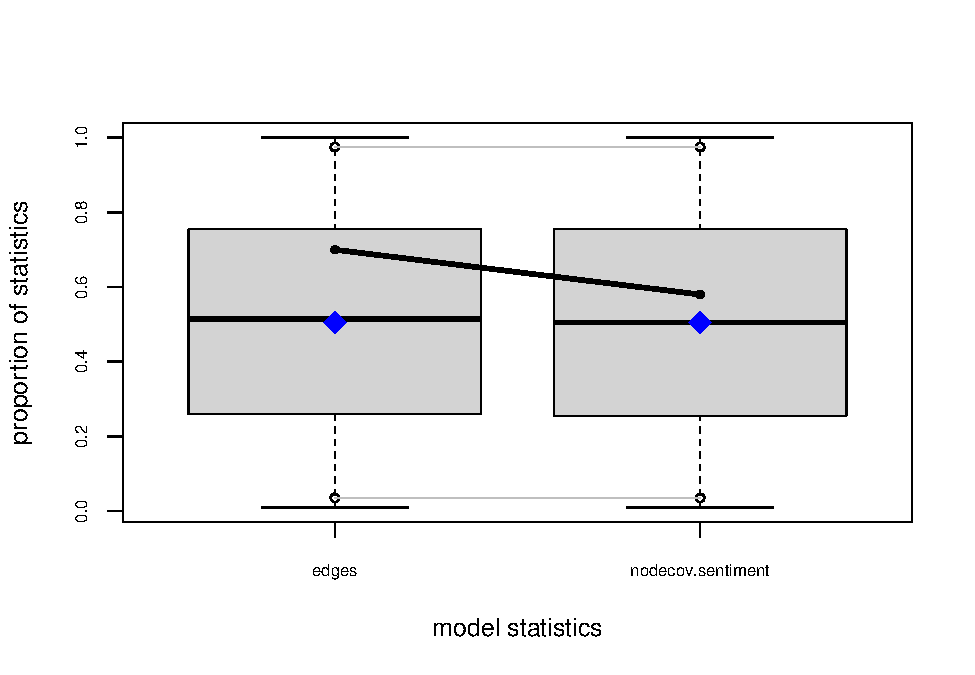
\includegraphics{E:/School/STA304/social_networks/outputs/report/report_files/figure-latex/unnamed-chunk-2-1.pdf} 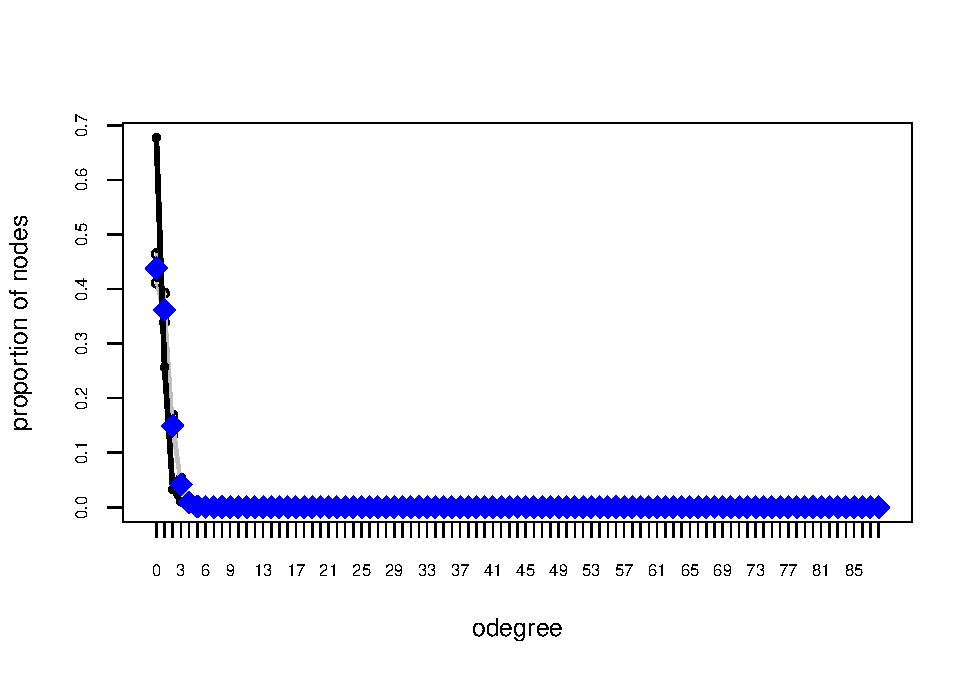
\includegraphics{E:/School/STA304/social_networks/outputs/report/report_files/figure-latex/unnamed-chunk-2-2.pdf} 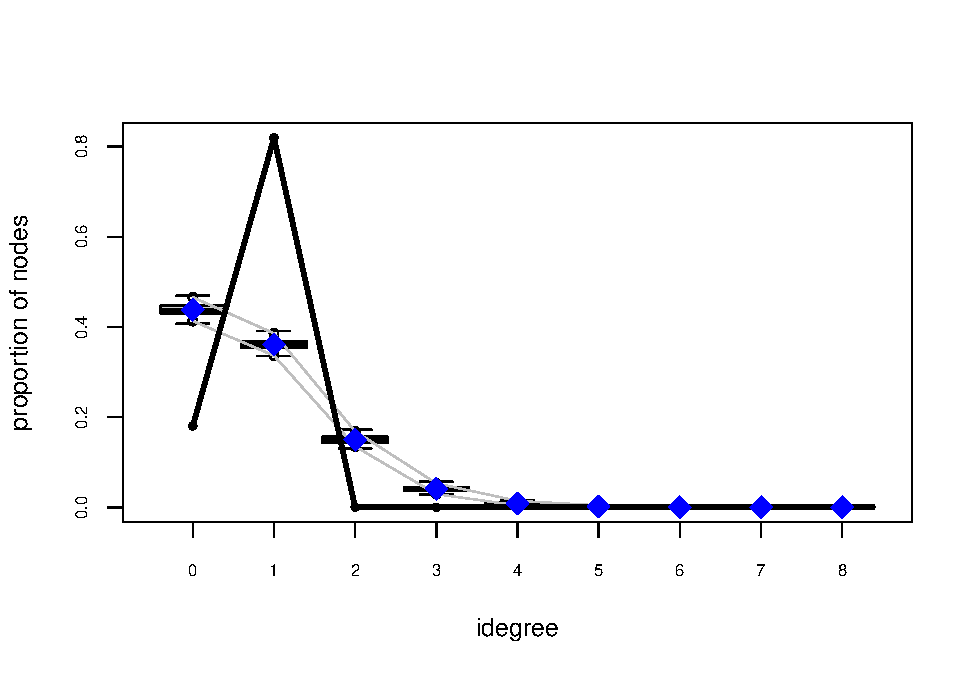
\includegraphics{E:/School/STA304/social_networks/outputs/report/report_files/figure-latex/unnamed-chunk-2-3.pdf} 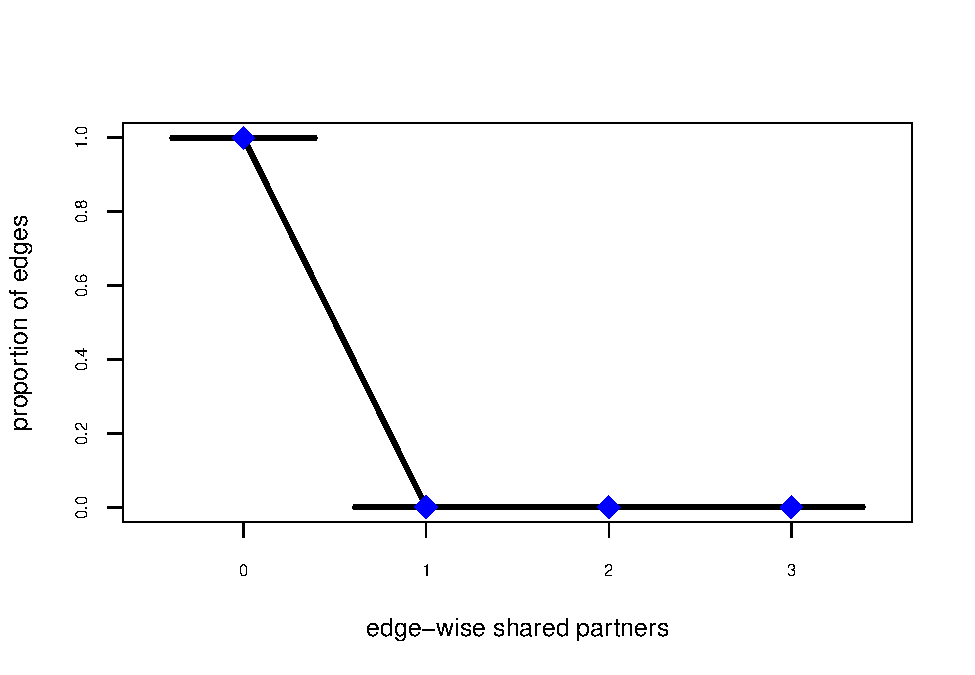
\includegraphics{E:/School/STA304/social_networks/outputs/report/report_files/figure-latex/unnamed-chunk-2-4.pdf} 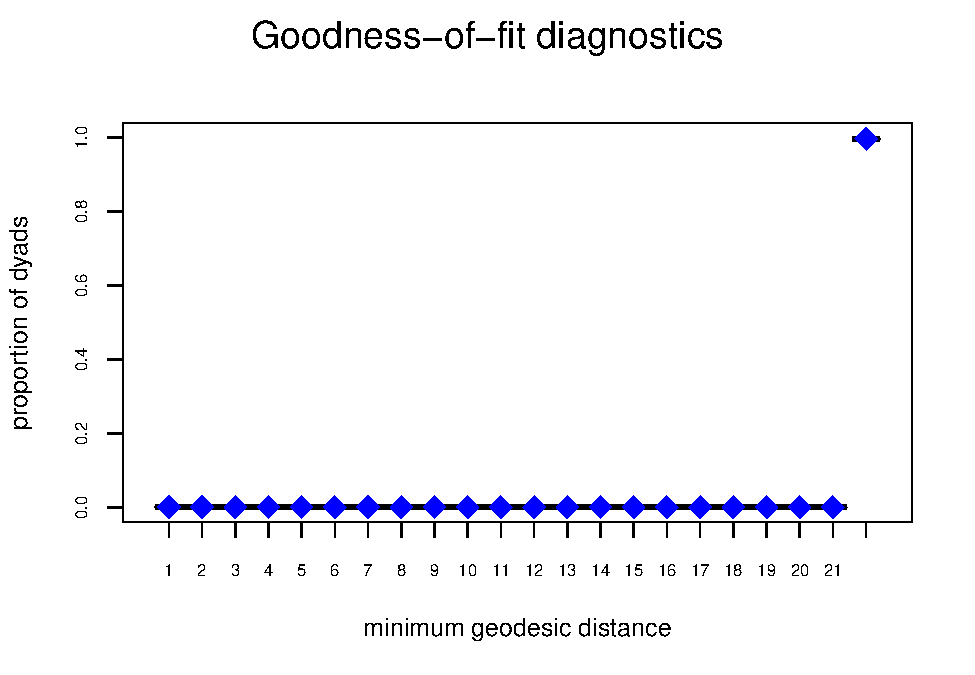
\includegraphics{E:/School/STA304/social_networks/outputs/report/report_files/figure-latex/unnamed-chunk-2-5.pdf}

\newpage

\hypertarget{appendix-b-data-sheet}{%
\section{Appendix B: Data sheet}\label{appendix-b-data-sheet}}

Extract of the questions from Gebru et al. (2021)

\textbf{Motivation}

\begin{enumerate}
\def\labelenumi{\arabic{enumi}.}
\tightlist
\item
  \emph{For what purpose was the dataset created? Was there a specific task in mind? Was there a specific gap that needed to be filled? Please provide a description.}

  \begin{itemize}
  \tightlist
  \item
    The dataset was created in order to examine polarity in the online social media site, Reddit. It was constructed with sentiment labels obtained via Vader (Hutto and Gilbert 2014), and with the goal of reporesenting comments as a social network.
  \end{itemize}
\item
  \emph{Who created the dataset (for example, which team, research group) and on behalf of which entity (for example, company, institution, organization)?}

  \begin{itemize}
  \tightlist
  \item
    William Gerecke.
  \end{itemize}
\item
  \emph{Who funded the creation of the dataset? If there is an associated grant, please provide the name of the grantor and the grant name and number.}

  \begin{itemize}
  \tightlist
  \item
    There was no funding for the project.
  \end{itemize}
\end{enumerate}

\textbf{Composition}

\begin{enumerate}
\def\labelenumi{\arabic{enumi}.}
\tightlist
\item
  \emph{What do the instances that comprise the dataset represent (for example, documents, photos, people, countries)? Are there multiple types of instances (for example, movies, users, and ratings; people and interactions between them; nodes and edges)? Please provide a description.}

  \begin{itemize}
  \tightlist
  \item
    Instances of the dataset represent comments on the social media site Reddit.
  \end{itemize}
\item
  \emph{How many instances are there in total (of each type, if appropriate)?}

  \begin{itemize}
  \tightlist
  \item
    The size of the dataset varies, but is on the order of 100,000 instances.
  \end{itemize}
\item
  \emph{Does the dataset contain all possible instances or is it a sample (not necessarily random) of instances from a larger set? If the dataset is a sample, then what is the larger set? Is the sample representative of the larger set (for example, geographic coverage)? If so, please describe how this representativeness was validated/verified. If it is not representative of the larger set, please describe why not (for example, to cover a more diverse range of instances, because instances were withheld or unavailable).}

  \begin{itemize}
  \tightlist
  \item
    This is an extremely small sample, as Reddit has over 1 million comments per day (reddit 2011). The size of the sample was limited by computational constraints. The sample was gathered by randomly performing a breadth first search over the social network. Links to posts were gathered by collecting the most recent activity of users on a given post, and comments were gathered from the posts. Since the posts have high multiplicity with respect to linked posts, nodes in the network were added to a list, and selected at random when visiting a post.
  \end{itemize}
\item
  \emph{What data does each instance consist of? ``Raw'' data (for example, unprocessed text or images) or features? In either case, please provide a description.}

  \begin{itemize}
  \tightlist
  \item
    Each instance of the dataset contains:

    \begin{itemize}
    \tightlist
    \item
      \texttt{subreddit}: the community that it was posted under
    \item
      \texttt{author}: the user id of the account that posted the comment
    \item
      \texttt{id}: the id assigned to the specific comment
    \item
      \texttt{to\_id}: the id of the comment or post that the comment replied to
    \item
      \texttt{permalink}: the url to the post that the comment was posted under
    \item
      \texttt{timestamp}: the UTC timestamp that the comment was created at
    \item
      \texttt{body}: the raw text of the comment
    \item
      \texttt{sentiment}: a score between -1 and 1 that represents the sentiment of the comment as generated by Hutto and Gilbert (2014)
    \end{itemize}
  \end{itemize}
\item
  \emph{Is there a label or target associated with each instance? If so, please provide a description.}

  \begin{itemize}
  \tightlist
  \item
    There is no explicit label, the dataset is meant to provide a sample of the structure of online interactions.
  \end{itemize}
\item
  \emph{Is any information missing from individual instances? If so, please provide a description, explaining why this information is missing (for example, because it was unavailable). This does not include intentionally removed information, but might include, for example, redacted text.}

  \begin{itemize}
  \tightlist
  \item
    No data is missing from individual instances, as incomplete instances were dropped from the dataset. This was due to information appearing as \texttt{NULL} when scraped, or in some cases, http errors.
  \end{itemize}
\item
  \emph{Are relationships between individual instances made explicit (for example, users' movie ratings, social network links)? If so, please describe how these relationships are made explicit.}

  \begin{itemize}
  \tightlist
  \item
    Yes, each instance in the dataset contains the id of the media that it is a reply to. That is, each instance of the dataset represents an edge in a social network.
  \end{itemize}
\item
  \emph{Are there recommended data splits (for example, training, development/validation, testing)? If so, please provide a description of these splits, explaining the rationale behind them.}

  \begin{itemize}
  \tightlist
  \item
    There is no recommended splits, as the model used in this project had no need for partitioning the data.
  \item
    If the data is split, it is important to respect the underlying structure of the data, and a random split would most likely lead to inaccurate model metrics. For example, it is important not to include comments from the same comment chain in the training and test data sets.
  \end{itemize}
\item
  \emph{Are there any errors, sources of noise, or redundancies in the dataset? If so, please provide a description.}

  \begin{itemize}
  \tightlist
  \item
    Redundancies were removed in the cleaning process, but it is important to note that the sentiment is most likely fairly noisy. While sentiment prediction models are accurate when operating over text that strictly adheres to language standards, online communication is much more nuanced. Vader was specifically designed to work well in online scenarios, but still has challenges (Hutto and Gilbert 2014).
  \end{itemize}
\item
  \emph{Is the dataset self-contained, or does it link to or otherwise rely on external resources (for example, websites, tweets, other datasets)? If it links to or relies on external resources, a) are there guarantees that they will exist, and remain constant, over time; b) are there official archival versions of the complete dataset (that is, including the external resources as they existed at the time the dataset was created); c) are there any restrictions (for example, licenses, fees) associated with any of the external resources that might apply to a dataset consumer? Please provide descriptions of all external resources and any restrictions associated with them, as well as links or other access points, as appropriate.}

  \begin{itemize}
  \tightlist
  \item
    The dataset is self contains and can be viewed of a snapshot of the Reddit taken at the time that the dataset was created. It contains links to media hosted by Reddit that may not necessarily be valid in the future.
  \end{itemize}
\item
  \emph{Does the dataset contain data that might be considered confidential (for example, data that is protected by legal privilege or by doctor-patient confidentiality, data that includes the content of individuals' non-public communications)? If so, please provide a description.}

  \begin{itemize}
  \tightlist
  \item
    The dataset does not intentionally contain confidential data.
  \end{itemize}
\item
  \emph{Does the dataset contain data that, if viewed directly, might be offensive, insulting, threatening, or might otherwise cause anxiety? If so, please describe why.}

  \begin{itemize}
  \tightlist
  \item
    Yes, Reddit is a social media site that has a wide variety of communities, including communities that are offensive. There are also communities oriented towards viewers 18+ which contain explicit material. As such, comments contained in this dataset may be offensie or explicit.
  \end{itemize}
\item
  \emph{Does the dataset identify any sub-populations (for example, by age, gender)? If so, please describe how these subpopulations are identified and provide a description of their respective distributions within the dataset.}

  \begin{itemize}
  \tightlist
  \item
    The only sub populations identified by the dataset are the communities on the site Reddit, subreddits. Each comment in the dataset belongs to a subreddit, and is explicitly labelled.
  \end{itemize}
\item
  \emph{Is it possible to identify individuals (that is, one or more natural persons), either directly or indirectly (that is, in combination with other data) from the dataset? If so, please describe how.}

  \begin{itemize}
  \tightlist
  \item
    No.~While accounts are recorded, the accounts are anoymous unless someone intentionally published their personal information.
  \end{itemize}
\item
  \emph{Does the dataset contain data that might be considered sensitive in any way (for example, data that reveals race or ethnic origins, sexual orientations, religious beliefs, political opinions or union memberships, or locations; financial or health data; biometric or genetic data; forms of government identification, such as social security numbers; criminal history)? If so, please provide a description.}

  \begin{itemize}
  \tightlist
  \item
    Yes. There are many different subreddits, some of which are oriented towards sensitive topics. As such, the comments may contain sensitive material.
  \end{itemize}
\item
  \emph{Any other comments?}

  \begin{itemize}
  \tightlist
  \item
    There are no other comments.
  \end{itemize}
\end{enumerate}

\textbf{Collection process}

\begin{enumerate}
\def\labelenumi{\arabic{enumi}.}
\tightlist
\item
  \emph{How was the data associated with each instance acquired? Was the data directly observable (for example, raw text, movie ratings), reported by subjects (for example, survey responses), or indirectly inferred/derived from other data (for example, part-of-speech tags, model-based guesses for age or language)? If the data was reported by subjects or indirectly inferred/derived from other data, was the data validated/verified? If so, please describe how.}

  \begin{itemize}
  \tightlist
  \item
    The data was directly acquired from \url{http://reddit.com}, and sentiment abels were generated using Vader.
  \end{itemize}
\item
  \emph{What mechanisms or procedures were used to collect the data (for example, hardware apparatuses or sensors, manual human curation, software programs, software APIs)? How were these mechanisms or procedures validated?}

  \begin{itemize}
  \tightlist
  \item
    The data was collected using a script that visited links to posts, and scraped comments. The script used a useful API published by Reddit that allows json representation of any content on the site. It was assumed that the data returned by the API is accurate.
  \end{itemize}
\item
  \emph{If the dataset is a sample from a larger set, what was the sampling strategy (for example, deterministic, probabilistic with specific sampling probabilities)?}

  \begin{itemize}
  \tightlist
  \item
    The sampling strategy is analogous to randomly advancing a breadth first search over the social network. If each post is considered a node in a social network, a random node was chosen, comments were gathered from that node, and new nodes were discovered. New nodes were discovered by gathering recent posts that users had commented on for each user who commented onthe post being scraped.
  \end{itemize}
\item
  \emph{Who was involved in the data collection process (for example, students, crowdworkers, contractors) and how were they compensated (for example, how much were crowdworkers paid)?}

  \begin{itemize}
  \tightlist
  \item
    I was the only person involved in the data collection process and I was not compensated.
  \end{itemize}
\item
  \emph{Over what timeframe was the data collected? Does this timeframe match the creation timeframe of the data associated with the instances (for example, recent crawl of old news articles)? If not, please describe the timeframe in which the data associated with the instances was created.}

  \begin{itemize}
  \tightlist
  \item
    The timeframe that data was collected over was very narrow, because of computational limitations. The analyses performed in this report became computationally intractable even with datasets around 100,000 elements long. As such, only a small amount of data was gathered.
  \end{itemize}
\item
  \emph{Were any ethical review processes conducted (for example, by an institutional review board)? If so, please provide a description of these review processes, including the outcomes, as well as a link or other access point to any supporting documentation.}

  \begin{itemize}
  \tightlist
  \item
    There was no ethical review process.
  \end{itemize}
\item
  \emph{Did you collect the data from the individuals in question directly, or obtain it via third parties or other sources (for example, websites)?}

  \begin{itemize}
  \tightlist
  \item
    The data was obtained via the Reddit website.
  \end{itemize}
\item
  \emph{Were the individuals in question notified about the data collection? If so, please describe (or show with screenshots or other information) how notice was provided, and provide a link or other access point to, or otherwise reproduce, the exact language of the notification itself.}

  \begin{itemize}
  \tightlist
  \item
    There was no notification given about the data collection.
  \end{itemize}
\item
  \emph{Did the individuals in question consent to the collection and use of their data? If so, please describe (or show with screenshots or other information) how consent was requested and provided, and provide a link or other access point to, or otherwise reproduce, the exact language to which the individuals consented.}

  \begin{itemize}
  \tightlist
  \item
    Consent for data collection was not give, however the data was publicly available.
  \end{itemize}
\item
  \emph{If consent was obtained, were the consenting individuals provided with a mechanism to revoke their consent in the future or for certain uses? If so, please provide a description, as well as a link or other access point to the mechanism (if appropriate).}

  \begin{itemize}
  \tightlist
  \item
    N/A
  \end{itemize}
\item
  \emph{Has an analysis of the potential impact of the dataset and its use on data subjects (for example, a data protection impact analysis) been conducted? If so, please provide a description of this analysis, including the outcomes, as well as a link or other access point to any supporting documentation.}

  \begin{itemize}
  \tightlist
  \item
    No.
  \end{itemize}
\item
  \emph{Any other comments?}

  \begin{itemize}
  \tightlist
  \item
    No other comments.
  \end{itemize}
\end{enumerate}

\textbf{Preprocessing/cleaning/labeling}

\begin{enumerate}
\def\labelenumi{\arabic{enumi}.}
\tightlist
\item
  \emph{Was any preprocessing/cleaning/labeling of the data done (for example, discretization or bucketing, tokenization, part-of-speech tagging, SIFT feature extraction, removal of instances, processing of missing values)? If so, please provide a description. If not, you may skip the remaining questions in this section.}

  \begin{itemize}
  \tightlist
  \item
    Labelling was done using the Vader sentiment model.
  \end{itemize}
\item
  \emph{Was the ``raw'' data saved in addition to the preprocessed/cleaned/labeled data (for example, to support unanticipated future uses)? If so, please provide a link or other access point to the ``raw'' data.}

  \begin{itemize}
  \tightlist
  \item
    Yes, the raw data was preserved, and can be found in the project repositroy.
  \end{itemize}
\item
  \emph{Is the software that was used to preprocess/clean/label the data available? If so, please provide a link or other access point.}

  \begin{itemize}
  \tightlist
  \item
    The software is available in the project repository under scripts.
  \end{itemize}
\item
  \emph{Any other comments?}

  \begin{itemize}
  \tightlist
  \item
    No other comments.
  \end{itemize}
\end{enumerate}

\textbf{Uses}

\begin{enumerate}
\def\labelenumi{\arabic{enumi}.}
\tightlist
\item
  \emph{Has the dataset been used for any tasks already? If so, please provide a description.}

  \begin{itemize}
  \tightlist
  \item
    No, the dataset has not been used for any other tasks.
  \end{itemize}
\item
  \emph{Is there a repository that links to any or all papers or systems that use the dataset? If so, please provide a link or other access point.}

  \begin{itemize}
  \tightlist
  \item
    N/A
  \end{itemize}
\item
  \emph{What (other) tasks could the dataset be used for?}

  \begin{itemize}
  \tightlist
  \item
    The dataset could be used for a variety of tasks associated with sentiment expression in online communities, such as assessing overall sentiment in communities, or toxicity.
  \end{itemize}
\item
  \emph{Is there anything about the composition of the dataset or the way it was collected and preprocessed/cleaned/labeled that might impact future uses? For example, is there anything that a dataset consumer might need to know to avoid uses that could result in unfair treatment of individuals or groups (for example, stereotyping, quality of service issues) or other risks or harms (for example, legal risks, financial harms)? If so, please provide a description. Is there anything a dataset consumer could do to mitigate these risks or harms?}

  \begin{itemize}
  \tightlist
  \item
    No.
  \end{itemize}
\item
  \emph{Are there tasks for which the dataset should not be used? If so, please provide a description.}

  \begin{itemize}
  \tightlist
  \item
    The dataset should not be used to attempt to identify individuals from their online presence.
  \end{itemize}
\item
  \emph{Any other comments?}

  \begin{itemize}
  \tightlist
  \item
    No other comments.
  \end{itemize}
\end{enumerate}

\textbf{Distribution}

\begin{enumerate}
\def\labelenumi{\arabic{enumi}.}
\tightlist
\item
  \emph{Will the dataset be distributed to third parties outside of the entity (for example, company, institution, organization) on behalf of which the dataset was created? If so, please provide a description.}

  \begin{itemize}
  \tightlist
  \item
    It will be publicly available on GitHub.
  \end{itemize}
\item
  \emph{How will the dataset be distributed (for example, tarball on website, API, GitHub)? Does the dataset have a digital object identifier (DOI)?}

  \begin{itemize}
  \tightlist
  \item
    The dataset will be available on GitHub, but does not have a DOI.
  \end{itemize}
\item
  \emph{When will the dataset be distributed?}

  \begin{itemize}
  \tightlist
  \item
    The dataset will be available immediately.
  \end{itemize}
\item
  \emph{Will the dataset be distributed under a copyright or other intellectual property (IP) license, and/or under applicable terms of use (ToU)? If so, please describe this license and/ or ToU, and provide a link or other access point to, or otherwise reproduce, any relevant licensing terms or ToU, as well as any fees associated with these restrictions.}

  \begin{itemize}
  \tightlist
  \item
    The dataset will be available under the MIT licence.
  \end{itemize}
\item
  \emph{Have any third parties imposed IP-based or other restrictions on the data associated with the instances? If so, please describe these restrictions, and provide a link or other access point to, or otherwise reproduce, any relevant licensing terms, as well as any fees associated with these restrictions.}

  \begin{itemize}
  \tightlist
  \item
    No.
  \end{itemize}
\item
  \emph{Do any export controls or other regulatory restrictions apply to the dataset or to individual instances? If so, please describe these restrictions, and provide a link or other access point to, or otherwise reproduce, any supporting documentation.}

  \begin{itemize}
  \tightlist
  \item
    No.
  \end{itemize}
\item
  \emph{Any other comments?}

  \begin{itemize}
  \tightlist
  \item
    No other comments.
  \end{itemize}
\end{enumerate}

\textbf{Maintenance}

\begin{enumerate}
\def\labelenumi{\arabic{enumi}.}
\tightlist
\item
  \emph{Who will be supporting/hosting/maintaining the dataset?}

  \begin{itemize}
  \tightlist
  \item
    There will be no supporting maintenance.
  \end{itemize}
\item
  \emph{How can the owner/curator/manager of the dataset be contacted (for example, email address)?}

  \begin{itemize}
  \tightlist
  \item
    I can be contacted via email at \href{mailto:wlgfour@gmail.com}{\nolinkurl{wlgfour@gmail.com}}, or via the GitHub associated with this project.
  \end{itemize}
\item
  \emph{Is there an erratum? If so, please provide a link or other access point.}

  \begin{itemize}
  \tightlist
  \item
    No.
  \end{itemize}
\item
  \emph{Will the dataset be updated (for example, to correct labeling errors, add new instances, delete instances)? If so, please describe how often, by whom, and how updates will be communicated to dataset consumers (for example, mailing list, GitHub)?}

  \begin{itemize}
  \tightlist
  \item
    The dataset will not be updated.
  \end{itemize}
\item
  \emph{If the dataset relates to people, are there applicable limits on the retention of the data associated with the instances (for example, were the individuals in question told that their data would be retained for a fixed period of time and then deleted)? If so, please describe these limits and explain how they will be enforced.}

  \begin{itemize}
  \tightlist
  \item
    N/A
  \end{itemize}
\item
  \emph{Will older versions of the dataset continue to be supported/hosted/maintained? If so, please describe how. If not, please describe how its obsolescence will be communicated to dataset consumers.}

  \begin{itemize}
  \tightlist
  \item
    Yes, data files will not be deleted, and are available on GitHub which keep a history of all files committed.
  \end{itemize}
\item
  \emph{If others want to extend/augment/build on/contribute to the dataset, is there a mechanism for them to do so? If so, please provide a description. Will these contributions be validated/verified? If so, please describe how. If not, why not? Is there a process for communicating/distributing these contributions to dataset consumers? If so, please provide a description.}

  \begin{itemize}
  \tightlist
  \item
    Contributors are welcome to fork the associated repository on GitHub, and use the code or data presented in the repository.
  \end{itemize}
\item
  \emph{Any other comments?}

  \begin{itemize}
  \tightlist
  \item
    No other comments.
  \end{itemize}
\end{enumerate}

\newpage

\hypertarget{references}{%
\section*{References}\label{references}}
\addcontentsline{toc}{section}{References}

\hypertarget{refs}{}
\begin{CSLReferences}{1}{0}
\leavevmode\vadjust pre{\hypertarget{ref-keyToEnglish}{}}%
Candocia, Max. 2021. \emph{keyToEnglish: Convert Data to Memorable Phrases}. \url{https://CRAN.R-project.org/package=keyToEnglish}.

\leavevmode\vadjust pre{\hypertarget{ref-stringi}{}}%
Gagolewski, Marek. 2021. \emph{Stringi: Fast and Portable Character String Processing in r}. \url{https://stringi.gagolewski.com/}.

\leavevmode\vadjust pre{\hypertarget{ref-gebru2021datasheets}{}}%
Gebru, Timnit, Jamie Morgenstern, Briana Vecchione, Jennifer Wortman Vaughan, Hanna Wallach, Hal Daumé Iii, and Kate Crawford. 2021. {``Datasheets for Datasets.''} \emph{Communications of the ACM} 64 (12): 86--92.

\leavevmode\vadjust pre{\hypertarget{ref-statnet}{}}%
Handcock, Mark S., David R. Hunter, Carter T. Butts, Steven M. Goodreau, Pavel N. Krivitsky, and Martina Morris. 2018. \emph{Ergm: Fit, Simulate and Diagnose Exponential-Family Models for Networks}. The Statnet Project (\url{http://www.statnet.org}). \url{https://CRAN.R-project.org/package=ergm}.

\leavevmode\vadjust pre{\hypertarget{ref-purrr}{}}%
Henry, Lionel, and Hadley Wickham. 2020. \emph{Purrr: Functional Programming Tools}. \url{https://CRAN.R-project.org/package=purrr}.

\leavevmode\vadjust pre{\hypertarget{ref-ergm}{}}%
Hunter, David R., Mark S. Handcock, Carter T. Butts, Steven M. Goodreau, and Martina Morris. 2008. {``Ergm: A Package to Fit, Simulate and Diagnose Exponential-Family Models for Networks.''} \emph{Journal of Statistical Software} 24 (3): 1--29.

\leavevmode\vadjust pre{\hypertarget{ref-vader}{}}%
Hutto, Clayton, and Eric Gilbert. 2014. {``Vader: A Parsimonious Rule-Based Model for Sentiment Analysis of Social Media Text.''} In \emph{Proceedings of the International AAAI Conference on Web and Social Media}, 8:216--25. 1.

\leavevmode\vadjust pre{\hypertarget{ref-jsonlite}{}}%
Ooms, Jeroen. 2014. {``The Jsonlite Package: A Practical and Consistent Mapping Between JSON Data and r Objects.''} \emph{arXiv:1403.2805 {[}Stat.CO{]}}. \url{https://arxiv.org/abs/1403.2805}.

\leavevmode\vadjust pre{\hypertarget{ref-r}{}}%
R Core Team. 2021. \emph{R: A Language and Environment for Statistical Computing}. Vienna, Austria: R Foundation for Statistical Computing. \url{https://www.R-project.org/}.

\leavevmode\vadjust pre{\hypertarget{ref-reddit}{}}%
reddit. 2011. {``Reddit.''} \url{http://reddit.com}.

\leavevmode\vadjust pre{\hypertarget{ref-git}{}}%
{``Where the World Builds Software.''} n.d. \emph{GitHub}. \url{https://github.com/}.

\leavevmode\vadjust pre{\hypertarget{ref-stringr}{}}%
Wickham, Hadley. 2019. \emph{Stringr: Simple, Consistent Wrappers for Common String Operations}. \url{https://CRAN.R-project.org/package=stringr}.

\leavevmode\vadjust pre{\hypertarget{ref-tidyr}{}}%
---------. 2021. \emph{Tidyr: Tidy Messy Data}. \url{https://CRAN.R-project.org/package=tidyr}.

\leavevmode\vadjust pre{\hypertarget{ref-dplyr}{}}%
Wickham, Hadley, Romain François, Lionel Henry, and Kirill Müller. 2021. \emph{Dplyr: A Grammar of Data Manipulation}. \url{https://CRAN.R-project.org/package=dplyr}.

\leavevmode\vadjust pre{\hypertarget{ref-wyatt}{}}%
Wyatt, Danny, Tanzeem Choudhury, and Jeff Bilmes. 2009. {``Dynamic Multi-Valued Network Models for Predicting Face-to-Face Conversations.''} In \emph{NIPS Workshop on Analyzing Networks and Learning with Graphs}. Citeseer.

\end{CSLReferences}

\end{document}
